%optics
Optical fibers are widely used as a medium for telecommuniction and networking because of varity of advantages.It is flexible,especially permits transmission over longer distances and at higher bandwidths (data rates) than other forms of communication. The Fig.\ref{fig:opticfiber} presents a simplest optical fiber and how lights progate in the fiber. 

\begin{figure}[httbp]
\centering
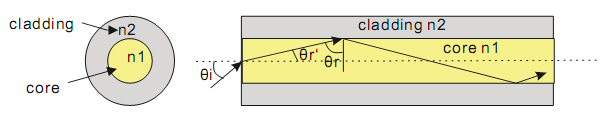
\includegraphics[width=0.8\textwidth]{bilder/opticfiber}
\caption{linght refraction in optic fibers}
\label{fig:opticfiber}
\end{figure}

Optical fiber typically consists of a transparent core with index $n1$ surrounded by a transparent cladding material with a lower index of refraction $n2$. The Light is kept in the core by total internal reflection. This causes the fiber to act as a waveguide.
The principle of the total reflection is explained in \cite{script_FT_TET} with Snell's law. In Fig.\ref{fig:totalreflection} linghts strike a boundary between two different isotropic media with respective refractive indices $n_{1}$ and $n_{2}$ ($n_{1}>n_{2}$), it behaves after Snell's law, which is presented in following mathematical fomular (\ref{eq:snell}).
\begin{figure}[httbp]
\centering
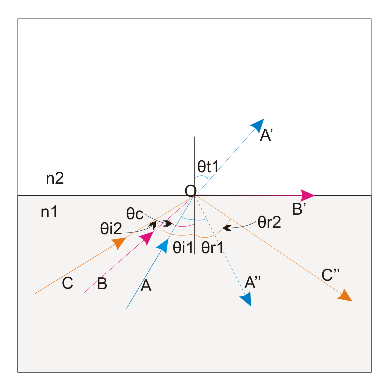
\includegraphics[width=0.6\textwidth]{bilder/totalreflection}
\caption{total reflection}
\label{fig:totalreflection}
\end{figure}

\begin{equation}
n_{1}sin\theta_{i}=n_{2}sin\theta_{t}
\label{eq:snell}
\end{equation}

$\theta_{t}$ is transmission angle or refraction angle.
At a small incidence angle $\theta_{i1}$ a light beam can pass through the boundary and bend to a new course at transmission angle $\theta_{t1}$ in the second meadium.
When the incidence angle is larger than a particular critical angle (\ref{eq:critical_angle}) with respect to the normal to the surface, no light can pass through and all of the light is reflected like (O-C''). In this case the value of $sin\theta_{t}$ in (\ref{eq:sin_transmission_angle}) become larger than one and he mathematical formular of the new transmission angle can be presented by a complex symble $\underline{\theta_{t}}$(\ref{eq:complex_transmission_angle}). $\underline{\theta_{t}}$ is not a real physical angle.

\begin{equation}
\theta_{c}=arcsin(\frac{n_{2}}{n_{1}})
\label{eq:critical_angle}
\end{equation}

\begin{equation}
sin\theta_{t}=\frac{n_{1}}{n_{2}}sin\theta_{i}
\label{eq:sin_transmission_angle}
\end{equation}

\begin{equation}
\underline{\theta_{t}}=\frac{\pi}{2}+j\gamma
\label{eq:complex_transmission_angle}
\end{equation}
with
\begin{equation}
sin\underline{\theta_{t}}=cosh\gamma=\frac{n{1}}{n_{2}}sin\theta_{i},\hspace{2cm}\hfill cos\underline{\theta_{t}}=jsinh\gamma=j\sqrt{cosh^2\gamma-1}
\label{eq:trangle_transmission_angle}
\end{equation}


%Numerical Apertur
Back to the Fig.\ref{fig:opticfiber} the incidence beam originate from the aire into the fiber. There is a maximus coupling angle,so that the beam can be guided under the total reflecting conditions. Its sinus value(\ref{eq:NA}) is called \textbf{Numerical Apertur(NA)}, which indicate the acceptable range of ray beams.

\begin{align}
sin\theta_{i}&=\frac{n_{1}}{n_{0}}sin(90^{o}-\theta_{c})=n_{1}cos\theta_{c} \nonumber\\
&=n_{1}\sqrt{1-sin^{2}\theta_{c}}=n_{1}\sqrt{1-\left(\frac{n_{2}}{n_{1}}\right)^2}=\sqrt{n^2_{1}-n^2_{2}}
\label{eq:NA}
\end{align}
